\chapter{Characterization of Exoplanet Systems Using Radial
  Velocities}\label{chap:boottran}

% boottran and TERMS and Katherina's long-period planet paper.

%---------------------------------------------------------------------------
\section{Introduction and Background}\label{boottran:sec:intro}

Extracting exoplanet signals from RV data is hard in many ways (see
Section~4 of \citealt{eprv2015} for a summary of the status of this
problem as of 2015). First, it can be hard to identify and quantify
stellar activity signals from planetary signals, and one of the
examples is the famous case of the GJ 581 system
\citep{2009A&A...507..487M, 2010ApJ...723..954V, 2013AN....334..616H,
  2014Sci...345..440R, 2015Sci...347.1080A,
  2015Sci...347.1080R}. Second, even with the definitive knowledge
that the RV signal is dominated by planets, it can still be
challenging if the planetary system is dynamically active, e.g., for
the case of the 55 Cnc system \citep{2014MNRAS.441..442N}, and
characterizing planetary orbits is a numerically and computationally
challenging problem \citep{2014ApJS..210...11N}. Third, even if the
star is RV quiet and the planetary system is dynamically quiet, and
all orbits can be described by simple Keplerian orbits, several
challenges remain for this parameter fitting or optimization
problem with complicated model selection scenarios: the number of
planets in the system can be hard to pin down
\citep{2015ApJ...814...12V, 2015A&A...584A..72M, 2016arXiv160205200J};
some orbits may not be well constrained and thus raise ambiguities
(e.g., circular orbits or eccentric; e.g.,
\citealt{2010ApJ...709..168A, 2013ApJS..208....2W,
  2015A&A...577A.103K}); and it can be computationally demanding.

In 2012, there were very few published codes on performing simple
Keplerian fit using RV data under the context of exoplanet detection
(i.e., handling multi-planets, data from multiple telescopes, etc.;
e.g., the systemic console, \citealt{2009PASP..121.1016M}), especially
ones that were easy to use. The \rvlin\ package by \cite{rvlin}
addresses the problem of simple Keplerian orbital fitting using
least-$\chi^2$ algorithm and exploiting the linear parameters (i.e.,
$K, \omega, \gamma$, and RV trend) to speed up the convergence. It
handles multi-planet systems and RV data from multiple telescopes, is
very easy to use (simple input requirements and easy commands; written
in IDL), and its typical time for convergence is within seconds. It is
fairly popular and has a large user group beyond the exoplanet
community (e.g., for binary stars and systems characterized using
astrometry, \citealt{2016AJ....151...57K}).

However, \rvlin\ does not provide estimates for uncertainties on
the best-fit parameters. This becomes a much desirable feature
especially for the Transit Ephemeris Refinement and Monitoring Survey
(TERMS) project \citep{Kane2009}. TERMS follows up RV detected
exoplanets with moderate separation from their bright, nearby host
stars (semi-major axis $>$ few hundredths of an AU) to search for
transiting ``warm" planets (as opposed to the Hot Jupiters), which are
unique and important targets for atmospheric characterization. TERMS
uses \rvlin\ for orbital parameter estimates, but only having the
best-fit Keplerian parameters will not suffice for transit prediction
and transit observation planning. A transit search can only be
feasible if the transit window is well constrained by the RV
data. Otherwise, more RVs need to be collected. As many of the TERMS
targets were reported in the literature a while ago, the predicted
transit ephemerides might have drifted from the true ones as the
predictive power of old RV data faded as time went by. Therefore,
estimating uncertainties on transit ephemerides becomes crucial for
the project.

With the purpose of calculating transit ephemerides and their
uncertainties for TERMS, and also to supplement \rvlin\ with a tool to
estimate uncertainties, I constructed the \boottran\ package, which
uses bootstrapping to calculate uncertainties for the Keplerian
parameters estimated by \rvlin. \boottran\ was heavily used in the
TERMS project and others (e.g., some of my co-authored publications:
\citealt{2013ApJ...768..155H, 2012ApJ...754...37D,
  2011ApJ...737...58K, 2011ApJ...735L..41K}; and
\citealt{2015ApJ...800...22F}). As of March 2016, \boottran\ and
\cite{wang2012} have received $\sim$30 citations. The statistical
justification and algorithm of \boottran\ is described in the next
section. The final section of this chapter describes my contributing
work on characterizing exoplanetary systems in in
\cite{2015ApJ...800...22F} and \cite{2013ApJ...768..155H} using other
tools besides \boottran. The next chapter, Chapter~\ref{chap:planets},
describes the planetary system around the star HD~37605, which serves
as an example of application of \rvlin\ and \boottran (similar with
other TERMS publications citing \citealt{wang2012} such as
\citealt{2012ApJ...754...37D}).


%---------------------------------------------------------------------------
\section{BOOTTRAN: Uncertainties for Orbital Parameters Estimated
  Using Radial Velocities}\label{boottran:sec:boottran}

{\it
  The following texts are originally published in the appendix of
  \cite{wang2012} in {\it ApJ}, and copy right belongs to IOP
  Publishing. They are used in this thesis with permission (with
  minor modification to fit in this chapter). 
}

We have constructed a package, \boottran, to calculate uncertainties
for Keplerian orbital parameter estimates\footnote{Through out this
  thesis, we refer to the ``{\it estimates} of the parameters'' (as
  distinguished from the ``true parameters'', which are not known and
  can only be estimated) simply as the ``parameters''.} and transit
mid-time $T_c$ via bootstrapping
\citep{1981,davison1997bootstrap}. \boottran\ is designed to calculate
error bars for transit ephemerides and the Keplerian orbital fit
parameters output by the RVLIN package\citep{rvlin}, but can also be a
stand-alone package. The two packages, \rvlin\ and \boottran, are
publicly available at http://exoplanets.org/code/ and the
Astrophysical Source Code Library (ASCL.net). Thanks to the simple
concept of bootstrapping, it is computationally very time-efficient
and easy to use.

The basic idea of bootstrap is to resample based on original data
to create bootstrap samples (multiple data replicates); then for
each bootstrap sample, derive orbital parameters or transit parameters
through orbital fitting and calculation. The ensemble of parameters
obtained in this way yields the approximate sampling distribution for
each estimated parameter. The standard deviation of this sampling
distribution is the standard error for the estimate.

We caution the readers here that there are regimes in which the
``approximate sampling distribution" (a frequentist's concept) is not
an estimate of the posterior probability distribution (a Bayesian
concept), and there are regimes (e.g., when limited sampling affects
the shape of the $\chi^2$ surface) where there are qualitative
differences and the bootstrap method dramatically underestimates
uncertainties \citep[e.g., long-period planets when the observations
  are not yet sufficient to pin down the orbital
  period;][]{Ford2005,Bender2012}. In situations with sufficient RV
data, good phase coverage, a sufficient time span of observations and
a good orbital fit, bootstrap often gives a useful estimate of the
parameter uncertainties. For the data considered in
Chapter~\ref{chap:planets} \citep{wang2012}, it was not obvious that
the bootstrap uncertainty estimate would be accurate, as the time span
of observations is only slightly longer than the orbital period of
planet $c$. Nevertheless, we find good agreement between the
uncertainty estimates derived from bootstrap and MCMC calculations in
\cite{wang2012}.

The radial velocity data are denoted as $\lbrace \vec{t},\ \vec{v},\ \vec{\sigma}
\rbrace$, where each $t_i$, $v_i$, $\sigma_i$ represents radial
velocity $v_i$ observed at time (BJD) $t_i$ with velocity uncertainty
$\sigma_i$. Extreme outliers should be rejected in order to preserve the
validity of our bootstrap algorithm. We first derive our estimates for
the true orbital parameters from the original RV data via orbital fitting,
using the RVLIN package: \beq \vec{\beta}
= \mu(\vec{t},\ \vec{v},\ \vec{\sigma}), \eeq where $\vec{\beta}$ is
the best fitted orbital parameters\footnote{As described in \S
  \ref{sec:fit}, this includes the $P$, $T_p$, $K$, $e$, and $\omega$
  for each planet, as well as $\gamma$, $\mbox{d}v/\mbox{d}t$ (if
  applicable), and velocity offsets between instruments/telescopes (if
  applicable) for the system.}. From $\vec{\beta}$, we derive $\lbrace
\vec{t},\ \vec{v}_{best}(\vec{\beta}) \rbrace$, the best-fit model
(here $\vec{t}$ are treated as predictors and thus fixed). Then we can
begin resampling to create bootstrap samples.

Our resampling plan is model-based resampling, where we draw from the
residuals against the best-fit model. For data that come from the
same instrument or telescope, in which case no instrumental offset
needs to be taken into account, we simply draw from all residuals,
$\lbrace \vec{v}-\vec{v}_{best} \rbrace$, with equal probability for
each $(v_i - v_{best,i})$. This new ensemble of residuals, denoted as
${\vec{r^*}}$, is then added to the best-fit model $\vec{v}_{best}$ to
create one bootstrap sample, $\vec{v^*}$ \footnote{We simply use the
  raw residual instead of any form of modified residual, because the
  RV data for any single instrument or telescope are usually close
  enough to homoscedasticity.}. Associated with ${\vec{r^*}}$, the
uncertainties $\vec{\sigma}$ are also re-assigned to $\vec{v^*}$ --
that is, if $v_j - v_{best,j}$ is drawn as $r_k$ and added to $v_k$ to
generate $v^*_k$, then the uncertainty for $v^*_k$ is set to be
$\sigma_j$.

For data that come from multiple instruments or multiple
telescopes, we incorporate our model-based resampling plan to include
stratified sampling. In this case, although data from each instrument
or telescope are close to homoscedastic, the entire set of data are
usually highly heteroscedastic due to stratification in
instrument/telescope radial velocity precision. Therefore, the
resampling process is done by breaking down the data into different
groups, $\lbrace \vec{v_1},\ \vec{v_2},\ \ldots \rbrace$, according to
instrument and/or telescope, and then resample within each
subgroup of data with the algorithm described in last paragraph. The bootstrap
sample is then $\vec{v^*} = \lbrace \vec{v^*}_1,\ \vec{v^*}_2,\ \ldots
\rbrace$.

To construct the approximate sampling distribution of the orbital
parameter estimates $\vec{\beta}$, we compute \beq \vec{\beta^*} =
\mu(\vec{t},\ \vec{v^*},\ \vec{\sigma^*}) \eeq for each bootstrap
sample, $\lbrace \vec{t},\ \vec{v^*},\ \vec{\sigma^*} \rbrace$. The
sampling distribution for each orbital parameter estimate $\beta_i$
can be constructed from the multiple sets of $\vec{\beta^*}$
calculated from multiple bootstrap samples
($\vec{\beta^*}^{(1)},\ \vec{\beta^*}^{(2)},\ \ldots$ from
$\vec{v^*}^{(1)},\ \vec{v^*}^{(2)},\ \ldots$). The standard errors for
$\vec{\beta}$ are simply the standard deviations of the sampling
distributions\footnote{The standard deviation of a sampling
  distribution is estimated in a robust way using the IDL function
  {\it robust\_sigma}, which is written by H. Fruedenreich based on
  the principles of robust estimation outlined in \cite{1983ured.book.....H}.}.

The sampling distribution of the estimated transit mid-time, $T_c$, is
calculated likewise. Here $T_c$ is the transit time for a certain
planet of interest in the system, and is usually specified to be the first
transit after a designated time $T$.  However, the situation is
complicated by the periodic nature of $T_c$. Our approach is to first
calculate, based on the original RV data, $T_{c0}$, the estimated
mid-time of the first transit after time $T_0$ (an arbitrary time
within the RV observation time window of $[\min(\vec{t}),\ \max(\vec{t})]$; $T_{c0}$ 
is also within this window).
Then
\beq
T_c = N\cdot P + T_{c0},
\eeq
where $P$ is the best-estimated period for this planet of interest,
and $N$ is the smallest integer that is larger than $(T - T_{c0})/P$.
Next we compute $T_{c0}^*$ for each bootstrap sample $\lbrace
\vec{t},\ \vec{v^*},\ \vec{\sigma^*} \rbrace$. Given that within the
time window of radial velocity observations
($[\min(\vec{t}),\ \max(\vec{t})]$), the phase of the planet should be
known well enough, it is fair to assume that $T_{c0}$ is an unbiased
estimator of the true transit mid-time. Therefore we assert that
$T_{c0}^*$ has to be well constrained and within the range of
$[T_{c0}-P^*/2,\ T_{c0}+P^*/2]$, where $P^*$ is the period estimated from
this bootstrap sample. If not, then we subtract or add multiple
$P^*$'s until $T_{c0}^*$ falls within the range. Then naturally
\beq
T_c^* = N\cdot P^* + T_{c0}^*.
\eeq
The ensemble of $T_c^*$'s gives the sampling distribution of $T_c$
and its standard error. Note that $T_c^*$ is not necessarily within
the rage of $[T_{c}-P/2,\ T_{c}+P/2]$.

Provided with the stellar mass $M_\star$ and its uncertainty, we
calculate, for each planet in the system, the standard errors for the
semi-major axis $a$ and the {\it minimum mass} of the planet $M_{\rm
  p,min}$ (denoted as $\msini$ in the main text as commonly seen in
literature, but this is a somewhat imprecise notation). As the first
step, the mass function is calculated for the best-fit $\vec{\beta}$
and each bootstrap sample $\vec{\beta^*}$,
\beq
f(P,K,e) = \frac{P K^3
  (1-e)^{3/2}}{2\pi G} = \frac{(M_p\cdot \sin i)^3}{(M_\star+M_p)^2}.
\eeq
The sampling distribution of $f(P,K,e)$ then gives the standard error
of the mass function. The minimum mass of the planet $M_{\rm p,min}$ 
is then calculated by assuming $\sin{i}=1$ and solving for $M_p$.
Standard error of $M_{\rm p,min}$ is derived through simple
propagation of error, as the covariance between $M_\star$ and
$f(P,K,e)$ is probably negligible.

For the semi-major axis $a$,
\beq
a^3 = \frac{P^2 G
  (M_\star+M_p)}{4\pi^2} \approx \frac{P^2 G (M_\star + M_{\rm p,min})}{4\pi^2}.
\eeq
The standard error of $P^2$ is calculated from its bootstrap sampling
distribution, and via simple propagation of error we obtain the
standard error of $a$ (neglecting covariance between $P^2$, $M_{\rm
  p,min}$, and $M_\star$).


%---------------------------------------------------------------------------
\section{Other Works on Characterization of Planetary Systems}

This section highlights my contributing work in
\cite{2015ApJ...800...22F} and \cite{2013ApJ...768..155H} using other
tools instead of \boottran\ for characterization of planetary systems.

{\bf (1)} \cite{2015ApJ...800...22F} reports updates and/or new detections on
the planetary systems around eight stars using RV data (primarily
taken by \keck), including: orbit updates for HD 24040, HD 183263, HD
74156, and HD 187123; a newly detected linear trend in RV for the HD
66428 system; RV coverage for complete orbits for GJ 849$c$ and HD
217107$c$; detection of HD 145934$b$. The emphasis of the paper is on
detecting and characterizing long-period planets, which can be
challenging because some of the planets have orbital periods on a $\sim$10
year time scale and thus have relatively poor RV coverage. In such
cases, it is important to illustrate good constraints on orbital
properties to confirm detection of the planets. A very useful tool is
the ``Wright diagram" (as referred to by
\citealt{2014ApJ...785..126K}; see, e.g.,
\citealt{2009ApJ...699L..97W}). For example,
Figure~\ref{boottran:mmperplot} is an Wright diagram for HD 217107$c$,
which shows the $\chi^2$ surface ``marginalized" over $\msini$ and $P$
(each $\chi^2$ value is for a set of optimized parameters with fixed
$\msini$ and $P$; see Section~\ref{sec:fit} for more details). This
demonstrates that the mass of HD 217107$c$ is well constrained to
justify its planetary nature (nominally $<13\ \mjup$), and the period
is decently constrained even though the RV data barely covers one
orbital period for HD 217107$c$. Figure~11 in
\cite{2015ApJ...800...22F} serves the same purpose but for GJ 849$c$.

% see email from Stephen Kane on 1/18/2013 'TERMS HD28529 paper' for
% my contribution
% plots from ExoPlanet.../TERMS/38529/
{\bf (2)} \cite{2013ApJ...768..155H} reports the host star properties
and transit exclusion for the HD 38529 system. TERMS refined the
orbital parameters for HD 38529$b$ and $c$ using new and archival RV
data from \hrs, Lick/Hamilton, and \keck. See
Figure~\ref{boottran:rvplot} for the RV plot for this system (orbital
fitting and uncertainty estimates from \rvlin\ and \boottran). The RV
data also enabled us to test the hypothesis of a third planet in the
system speculated by \cite{2010AJ....139.1844B}, using Monte Carlo to
estimate the significance of potential periodic signals in the RV
residuals to the two-planet Keplerian solution.

{\it The texts below are from Section~3.4 of
  \cite{2013ApJ...768..155H} and were co-written by me and the second
  author Stephen R.\ Kane (with minor revisions for consistency with
  this chapter).}

The results of \cite{2010AJ....139.1844B} are utilized by the authors
to speculate on evidence for a third planet in the system of HD
38529. Thus we also consider this possibility from our analysis since
our RV data comprise a substantially larger dataset. As reported by
\cite{2010AJ....139.1844B}, a coplanary orbital solution is only
stable if the third planet has a period within the window of
$[33,445]$ days and an eccentricity of $<0.3$, or a period larger than
their RV data baseline ($>10$ years). For this reason, we focused our
search for the third planet within the period window of $[33,445]$
days, and constrained the eccentricity to be $<0.3$.

We first searched for strong periodic signals in the residuals of the
two-planet Keplerian solution by fitting sinusoids to the residuals at
different periods within $[33,445]$ days (with 0.4 day step in
period). The results are plotted in solid line in Figure~\ref{boottran:nod}. We then
estimated the false positive probability to see if any of the strong
peaks are significant enough. We define the false positive probability
for a peak with a certain amplitude $K'$ as the probability that a
signal with amplitude $\geq K'$ is generated by the residuals just by
chance. We generated 1000 sets of simulated residuals by scrambling
the true residuals (and their associated errors, with replacements),
and then searched for the peak with largest amplitude within the
$P=[33,445]$ day window for each of the 1000 sets. These 1000
amplitudes provide approximately the distribution of amplitudes
arising purely from random noise in the residuals. Any peak in
Figure~\ref{boottran:nod} that has an amplitude smaller than 950 (95\%) of these 1000
amplitudes is thus considered having false positive probability of
$>5\%$. This is marked by the top dashed line in Figure~\ref{boottran:nod}, and
similarly for the $10\%$ and $50\%$ lines.

As shown in Figure~\ref{boottran:nod}, no peak has a false positive probability of less
than 5\%, and two with less than 10\% at 119 days and 164 days. We see
no significant peak around 194 days as reported by
\cite{2010AJ....139.1844B}. We then performed 3-planet Keplerian fit
with our RV data within the $P=[33,445]$ day window and with the
constraint that the eccentricity must be smaller than 0.3. We found
that indeed the best-fit is near 164 days, with $e=0.3$ (also true if
we force the third planet to be on circular orbit; best-fit $e=0.99$
if no constraint on $e$ is required). The $\chi_{\nu}^2$ of this fit
is 9.58, and an F-test suggests that the 3-planet model provides a
better fit though having 5 more parameters. However, the RMS for this
fit is 11.92 m s$^{-1}$, i.e., adding a third planet does not reduce
the RMS of the fit. Combining with the fact that this signal at
$P=164$ days does not have lower than 5\% false positive probability,
we cannot conclude that our data have detected a third planet in the
HD 38529 system.

We note here that including or excluding this third planet does not
affect our transit exclusion analysis in the following sections,
because the changes in the orbital parameters for both HD 38529$b$ or
$c$, after adding the third planet, are smaller than their error bars.



\newpage

%----------------------------------------------------------------
% MMPER Plot
\begin{figure}
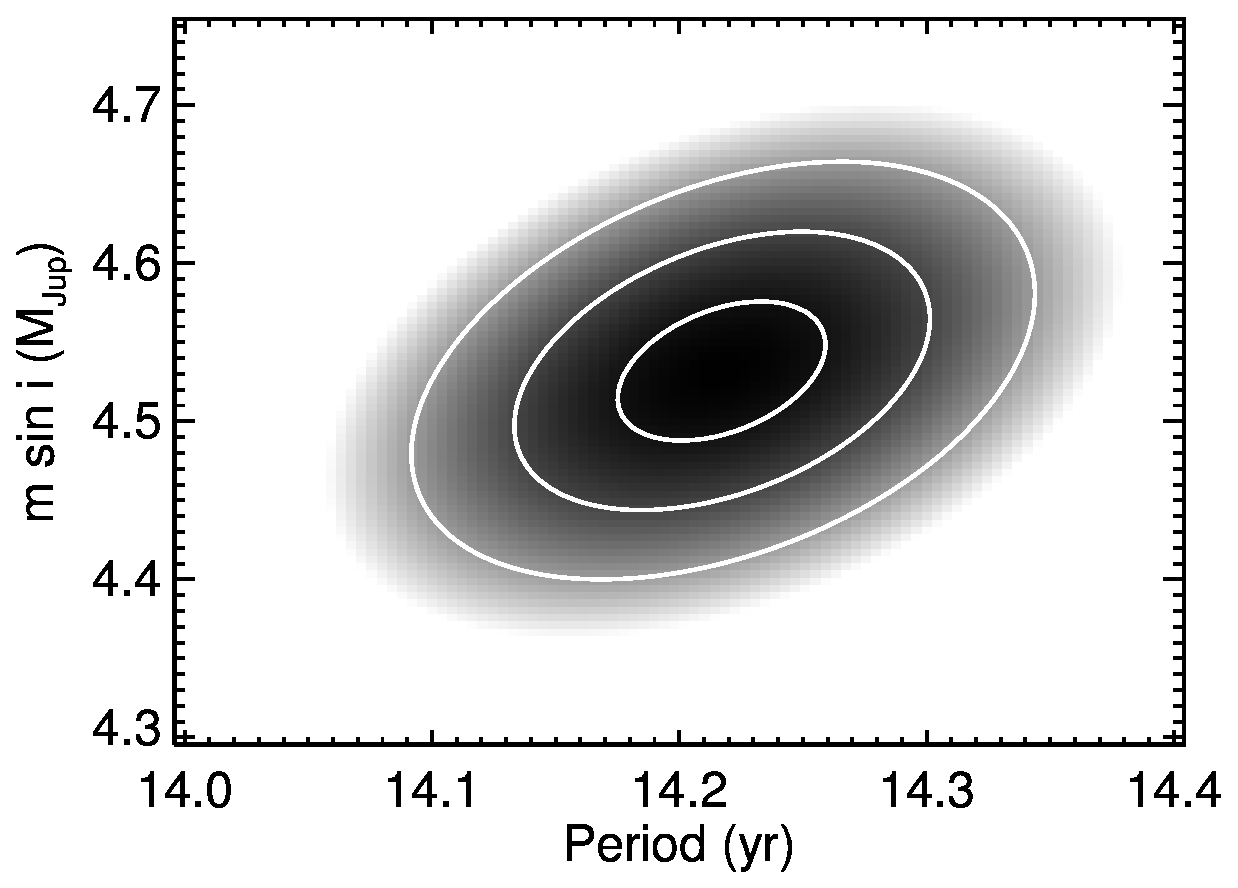
\includegraphics[scale=0.6]{boottran/feng2015-f9-217107.eps} 
\caption{Best-fit 100$\times$100 $\chi^2$ map for fixed values of $P_c$ and
  $M_c\sin{i_c}$ for HD 217107$c$. This confirms that the period and
  mass are well-constrained.  We have illustrated the contours of the
  1$\sigma$, 2$\sigma$, and 3$\sigma$ (defined by $\chi^2 =
  \chi^2_{\rm min} + \{2.30, 6.17, 11.8\}$) confidence levels, based on
  for the number of degrees of freedom in the problem
  \citep{2002nrca.book.....P}. The center and 1$\sigma$ limits in both
  parameters are consistent with the bootstrapping uncertainties for
  these parameters. This figure is published as Figure~9 in
  \cite{2015ApJ...800...22F} and was co-produced by me and the
  leading author Y.\ Katherina Feng.
\label{boottran:mmperplot}}
\end{figure}
%----------------------------------------------------------------


%----------------------------------------------------------------
% RV plot
\begin{figure}
\subfloat{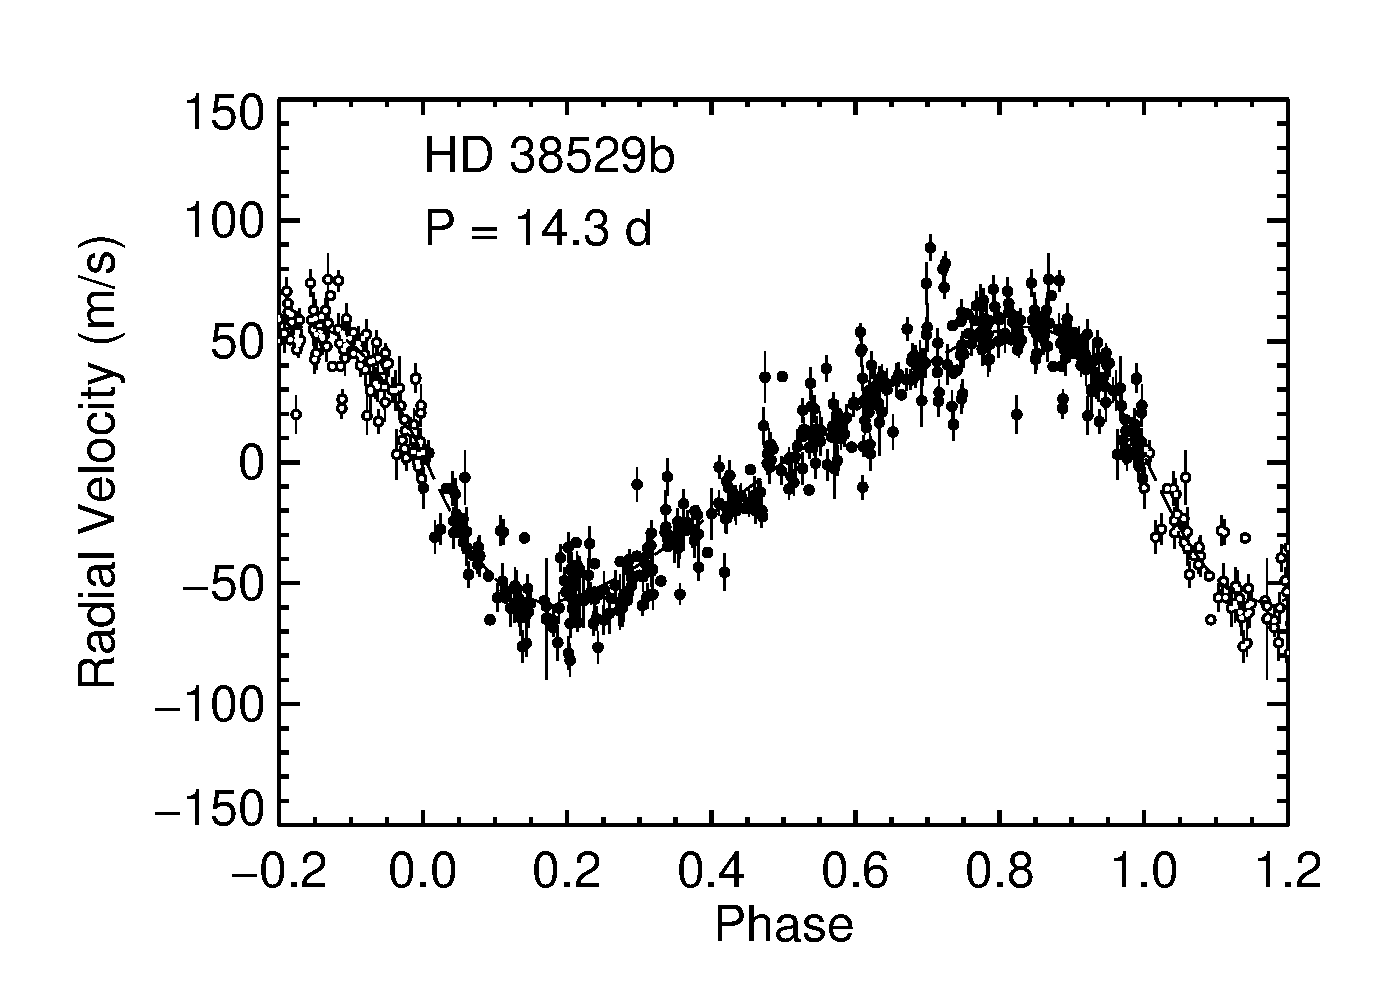
\includegraphics[scale=0.3]{boottran/38529_b.eps}}\
\subfloat{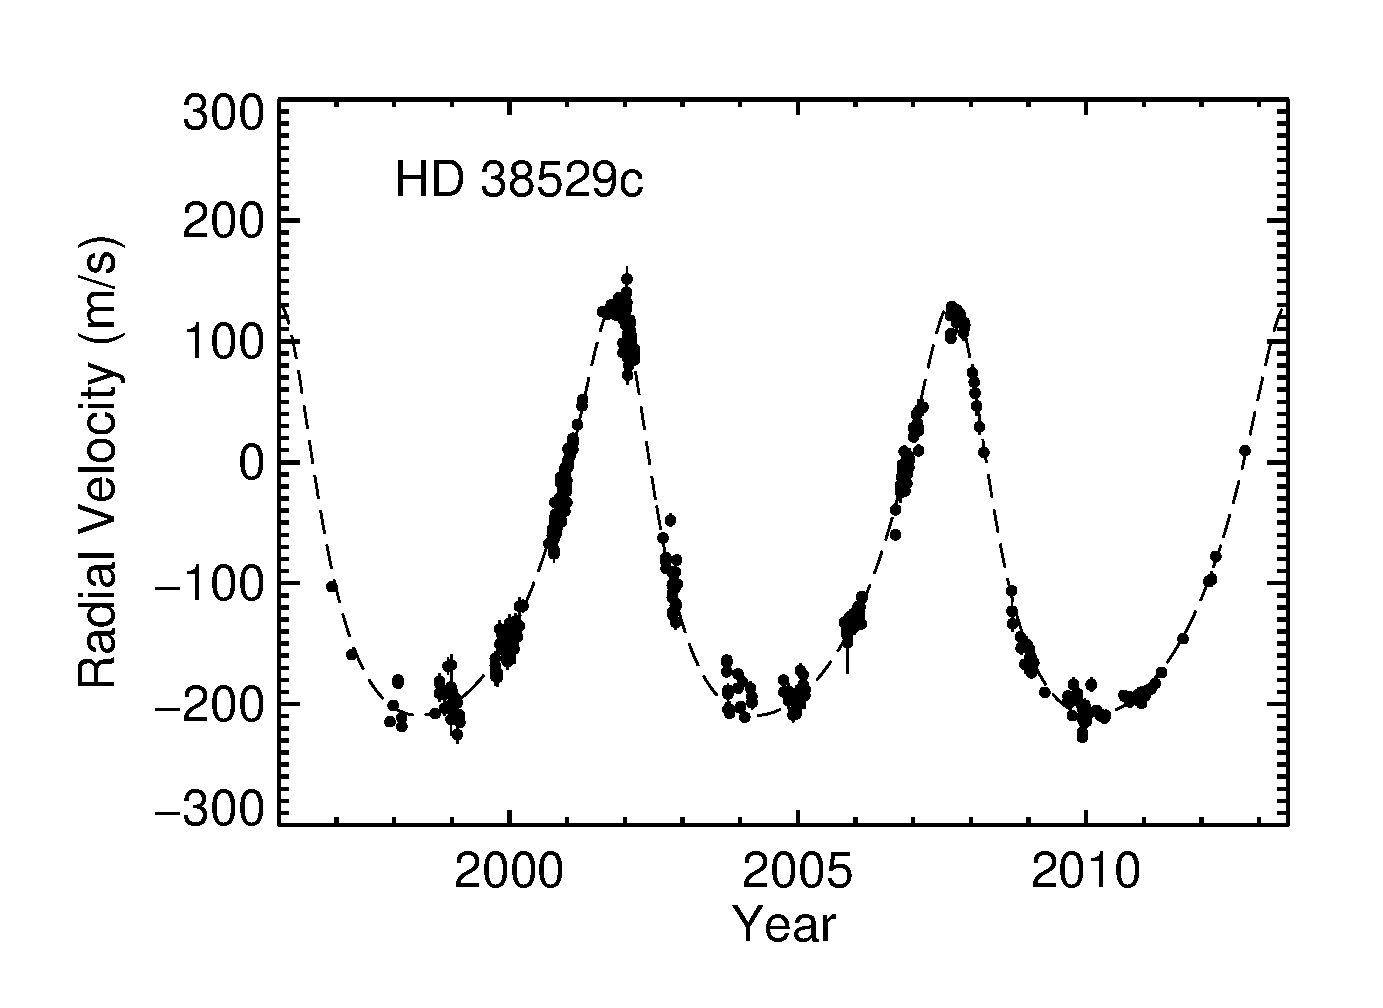
\includegraphics[scale=0.3]{boottran/38529_c.eps}}\
\centering
\subfloat{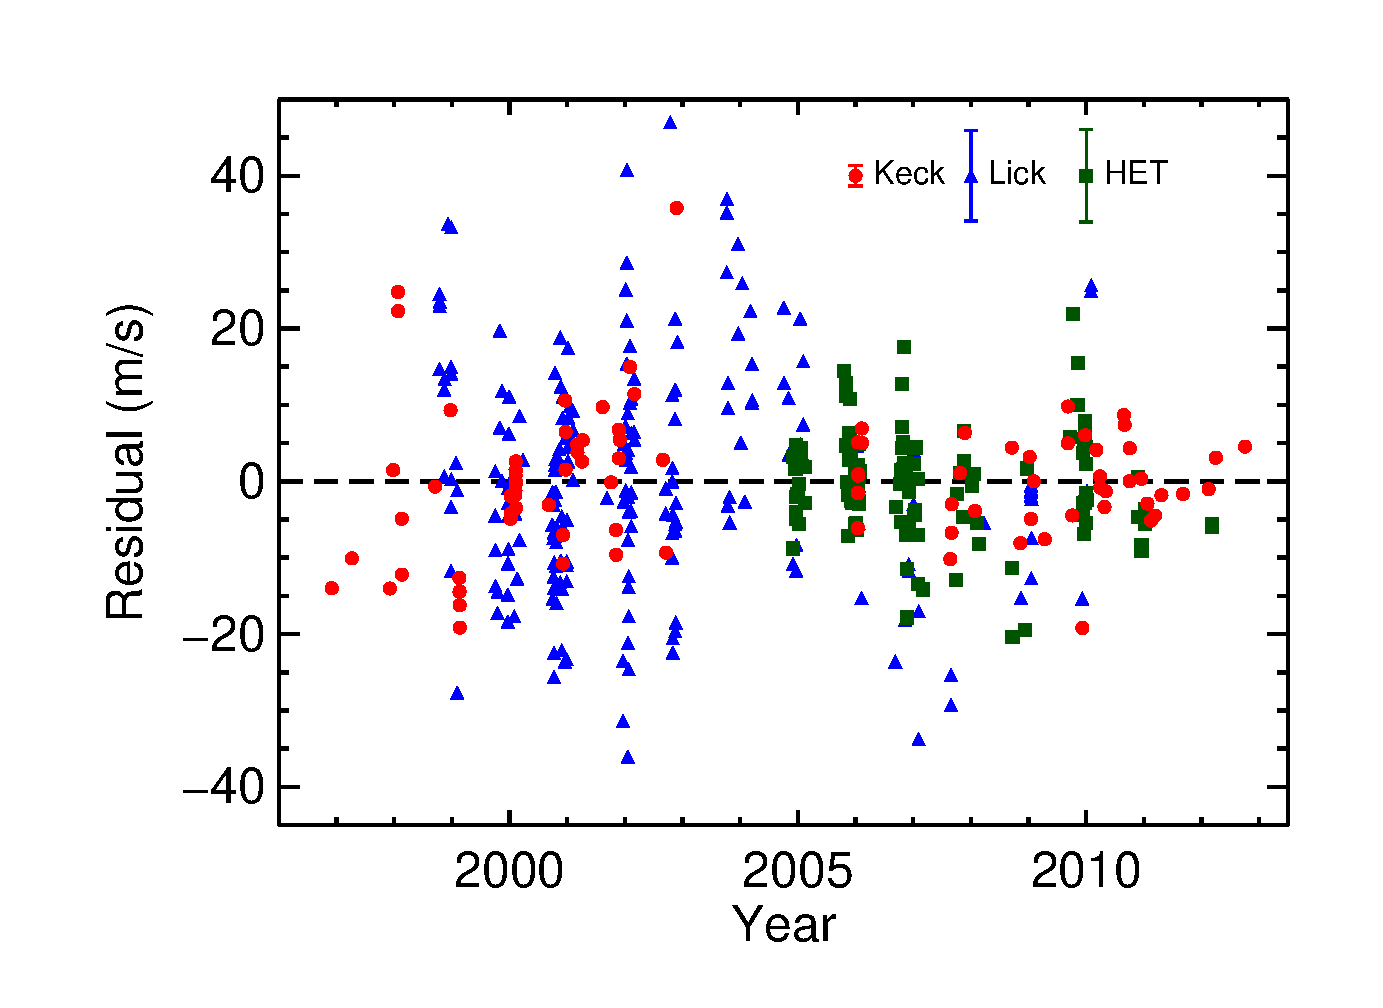
\includegraphics[scale=0.3]{boottran/38529_res.eps}}
\caption{Top two panels: radial velocity signal (black dots) induced
  by HD 38529$b$ and $c$, respectively, and the best-fit orbital
  solution (dashed line). Error bars shown are internal errors for
  each observation. The radial velocity signal for each planet was
  extracted by subtracting off the best-fit orbital velocities of the
  other planet from the total observed RVs. Bottom panel: residual
  velocities with respect to the best two-planet orbital solution. The
  red dots are for Keck data (data sets 3 and 4 in
  \cite{2013ApJ...768..155H}), the blue triangles are for Lick data
  (data sets 5 and 6), and the green squares are for the HET data
  (data sets 1 and 2). The typical size of internal error bars for
  each telescope ($\pm$ median internal errors) are plotted on the
  upper right of this panel. This figure is published as Figure~2 in
  \cite{2013ApJ...768..155H} and was made by me.
\label{boottran:rvplot}}
\end{figure}
%----------------------------------------------------------------


%----------------------------------------------------------------
% NOD plot
\begin{figure}
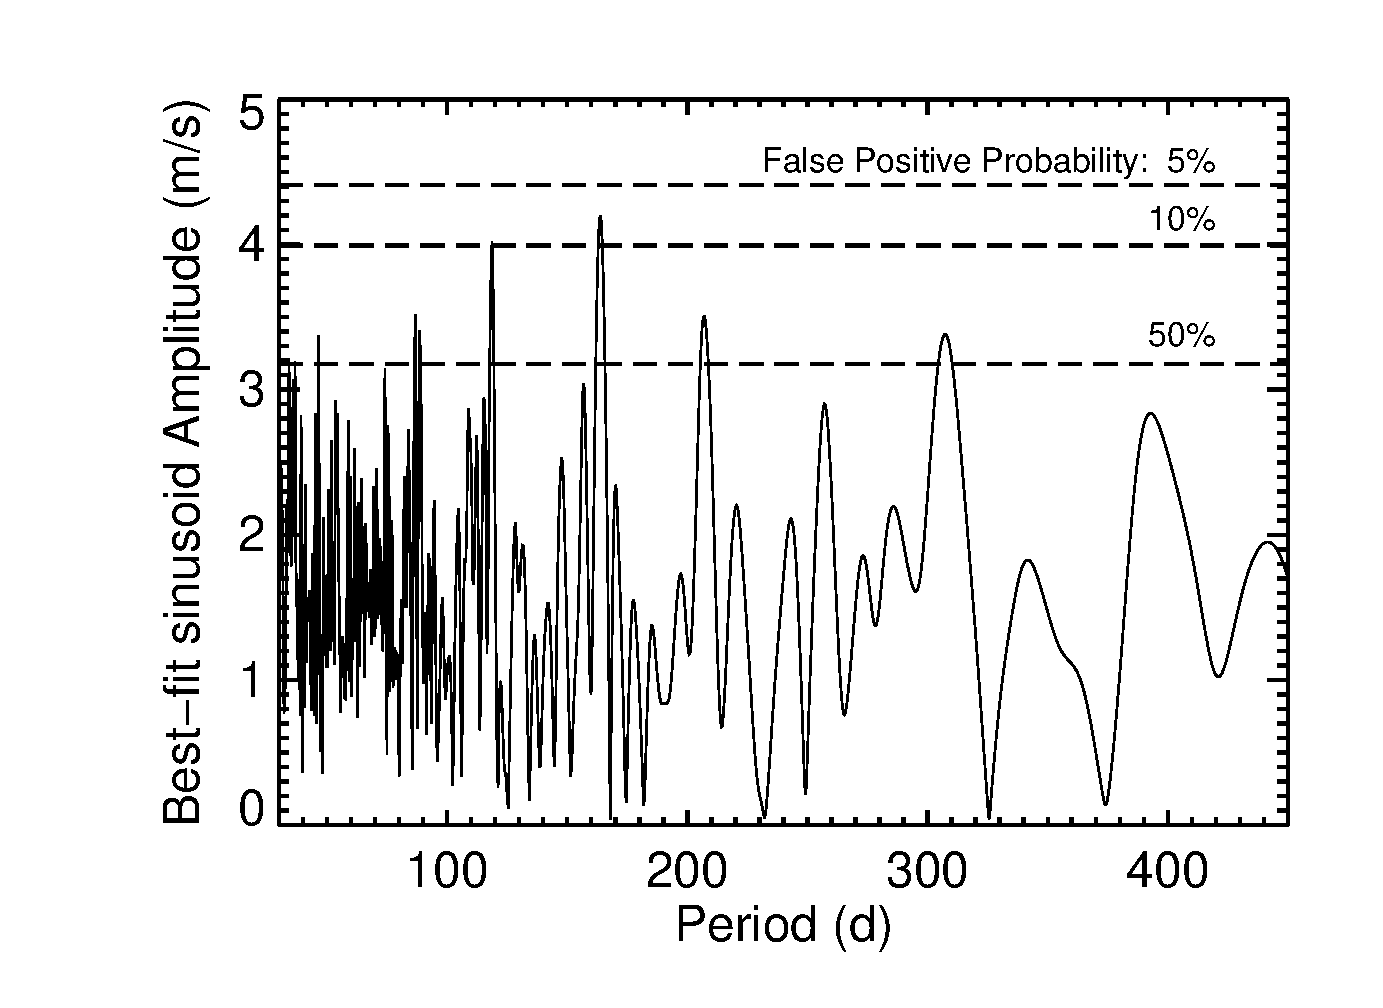
\includegraphics[scale=0.6]{boottran/nod.eps} 
\caption{Amplitude of best-fit sinusoids to the residuals of the
  two-planet Keplerian solution (solid line). Any peak in this period
  window that has amplitude larger than the top dashed line is
  considered to be significant for having $<5\%$ false positive
  probability. Similar meanings for the two lower dashed lines
  ($<10\%$ and $<50\%$). No period within this window has less than
  5\% false positive probability, and the two peaks with $<10\%$ false
  positive probability are at 119 days and 164 days. We see no
  significant peak around 194 days as reported by
  \cite{2010AJ....139.1844B}. This figure is published as Figure~3 in
  \cite{2013ApJ...768..155H} and was made by me.
\label{boottran:nod}}
\end{figure}
%----------------------------------------------------------------


